\section{MPI One-Sided Communication}
\subsection{Required submission files}
\begin{enumerate}
  \item \hl{The updated \emph{gauss.c} file.}

    \verb!Data/path/to/file!

  \item \hl{The new performance plots and description in the report.}

    References to figures here...

\end{enumerate}

\subsection{Questions}
\begin{enumerate}
  \item \hl{Which one-sided operations were used? Justify your choice.}

	We targeted the blocking \verb!MPI_Send! and \verb!MPI_Recv! functions passing pivot data for optimization for optimization.
	These were the most affected by the blocking operations and was the most likely to benefit from overlapping communication and computation.
    We decided to use the Post-Start-Wait-Complete methodology, which uses the following 
    MPI functions: \verb!MPI_Win_start!, \verb!MPI_Win_post!, \verb!MPI_Get! and \verb!MPI_Win_complete!. 
    This methodology allows the use of unique MPI communication groups---specifying the specific processes which are allowed to participate in a particular exposure/access epoch.
    This is useful for this use case as the communication of information only goes from processes with a lower rank number to processes with a higher rank number when distributing the pivot data.
    There is additionally a final aggregation phase where the computed information is passed back to process 0.
    However, the time associated with this phase is negligible in relation to the time spent communicating pivot data.
    We have decided to go with \verb!MPI_Get! function because it fits the purpose of distributing
    data from the process that had computed his part of pivoting to the rest.

  \item \hl{Was communication and computation overlap achieved? Use Vampir.}

    Yes it was achieved and it can be seen in Fig \ref{fig:vampir_haswell_one_sided} \& \ref{fig:vampir_sandy_one_sided}. We can clearly see in both examples that there is computation occuring as certain processes are waiting.
    \begin{figure}[h] % h=here, t=top, b=bottom, p=(extra)page, !=force
	\begin{center}
			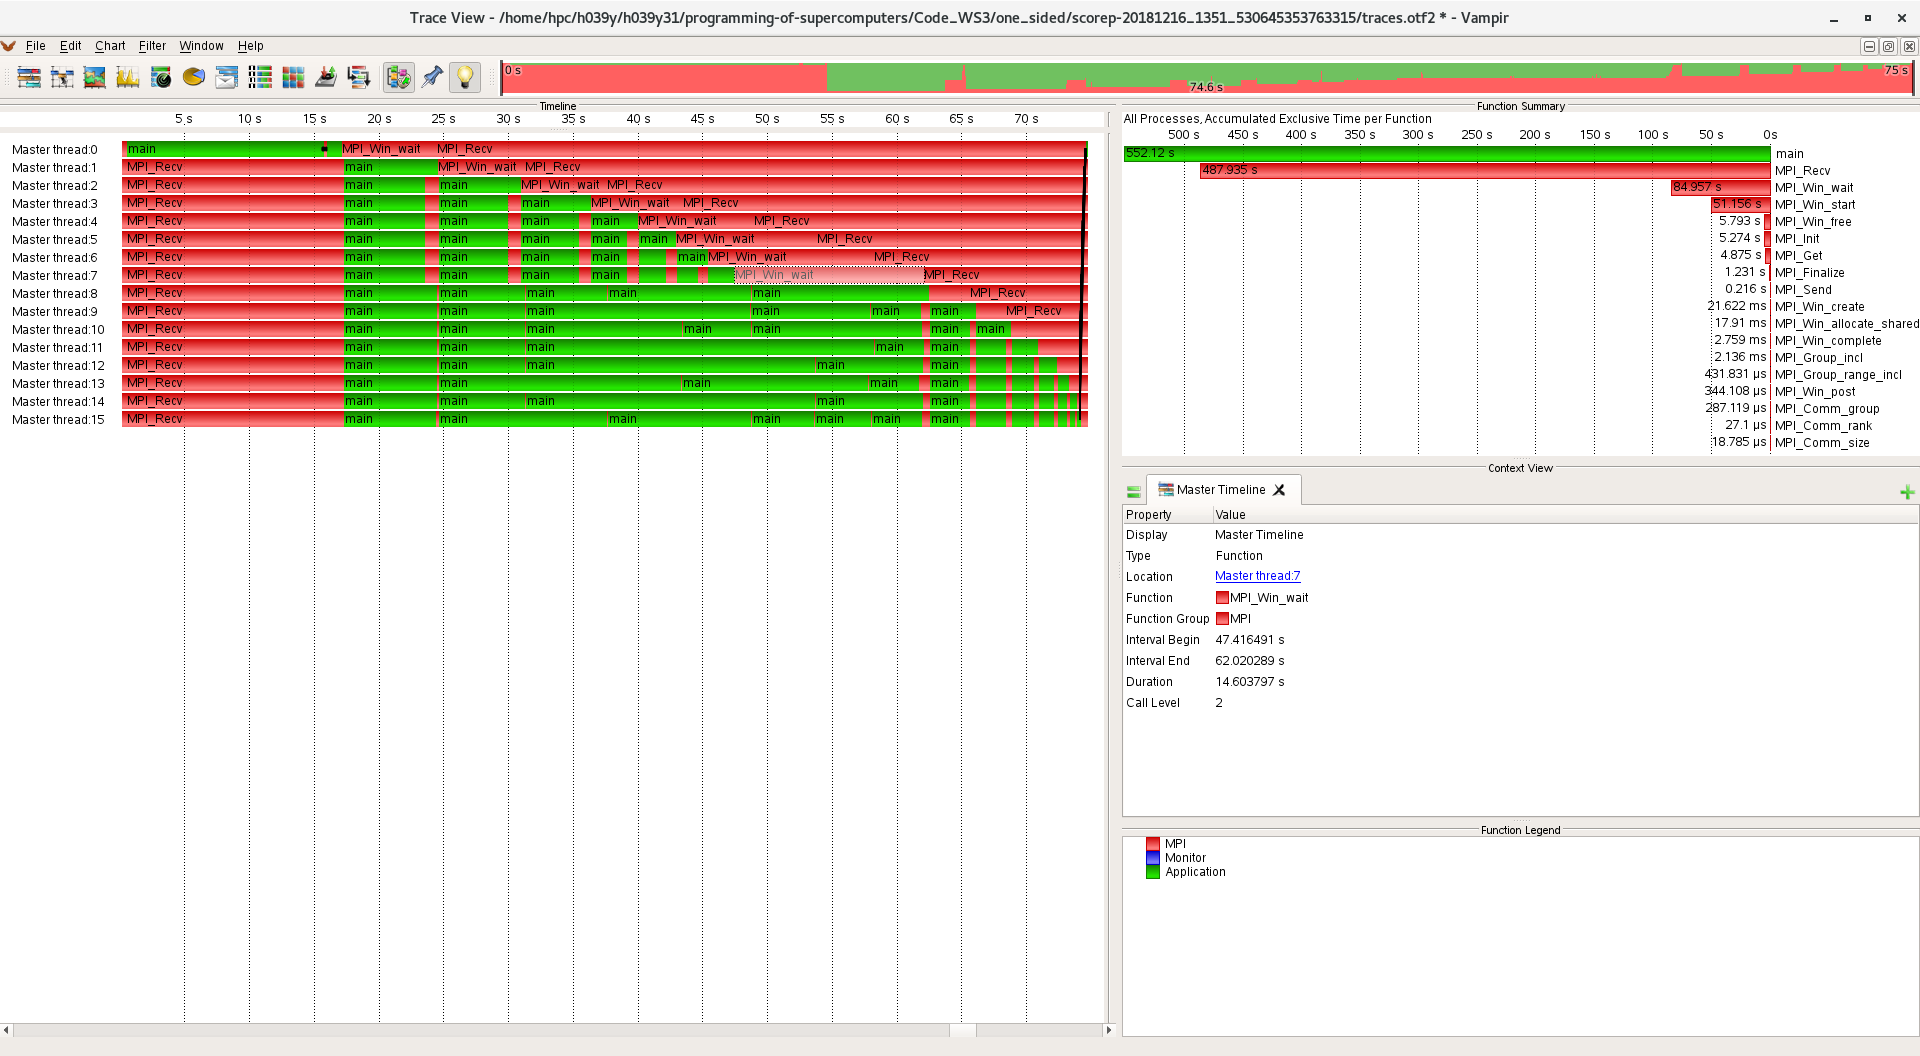
\includegraphics[width=.8\linewidth]{/one_sided/vampir_onesided_hw.png}
		\caption{Vampir output for One-Sided Communication, Haswell}
		\label{fig:vampir_haswell_one_sided}
	\end{center}
	\end{figure}
	
	    \begin{figure}[h] % h=here, t=top, b=bottom, p=(extra)page, !=force
	\begin{center}
			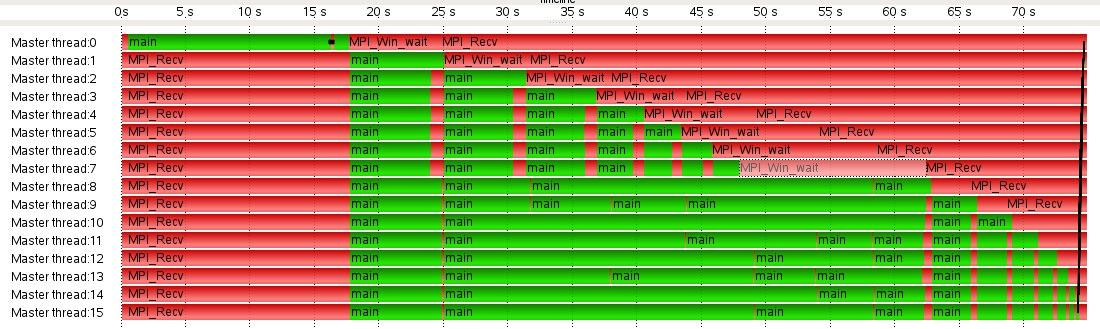
\includegraphics[width=.8\linewidth]{/one_sided/vampir_onesided_sb.jpg}
		\caption{Vampir output for One-Sided Communication, Sandy Bridge}
		\label{fig:vampir_sandy_one_sided}
	\end{center}
	\end{figure}

  \item \hl{Was a speedup observed versus the baseline for the Sandy Bridge and Haswell nodes?}

    Results performed on Haswell and Sandy Bridge for One-sided communication are almost the same.
  
    Despite the fact that overlap of the communication and computation was achieved, overall time
    was even worse than for baseline. This was due the fact that processors with a higher rank number 
    had long computation times. Therefore, they become a bottleneck
    for this implementation. This is expected since these portions will perform the Gaussian Elimination
    steps more times than the processes with lower ranks.
    
    Additionally, the Guassian Elimination algorithm is inherently sequential and hard to load balance
    properly---resulting in the observed phenomenon where certain processes perform far more compuation
    than others.
    
    We can view the results comparing the computational time and MPI time of the Baseline and the One-Sided communication below.
    
    	\begin{figure}[h] % h=here, t=top, b=bottom, p=(extra)page, !=force
		\hspace*{-0.25\linewidth}\begin{tabular}{cc}
			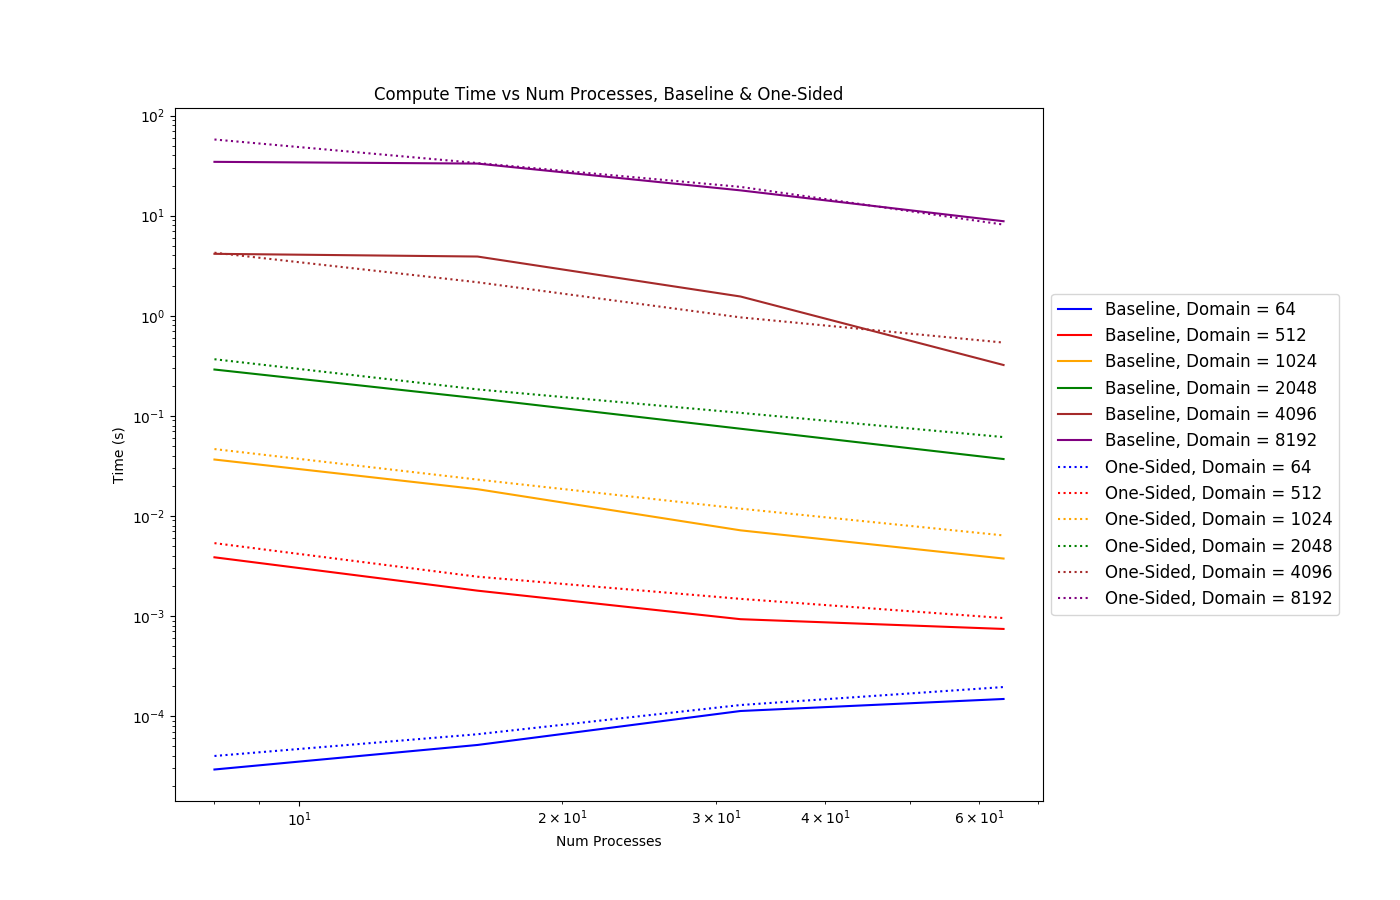
\includegraphics[width=.75\linewidth]{one_sided/compute_multdomain_haswell_os_baseline.png} & 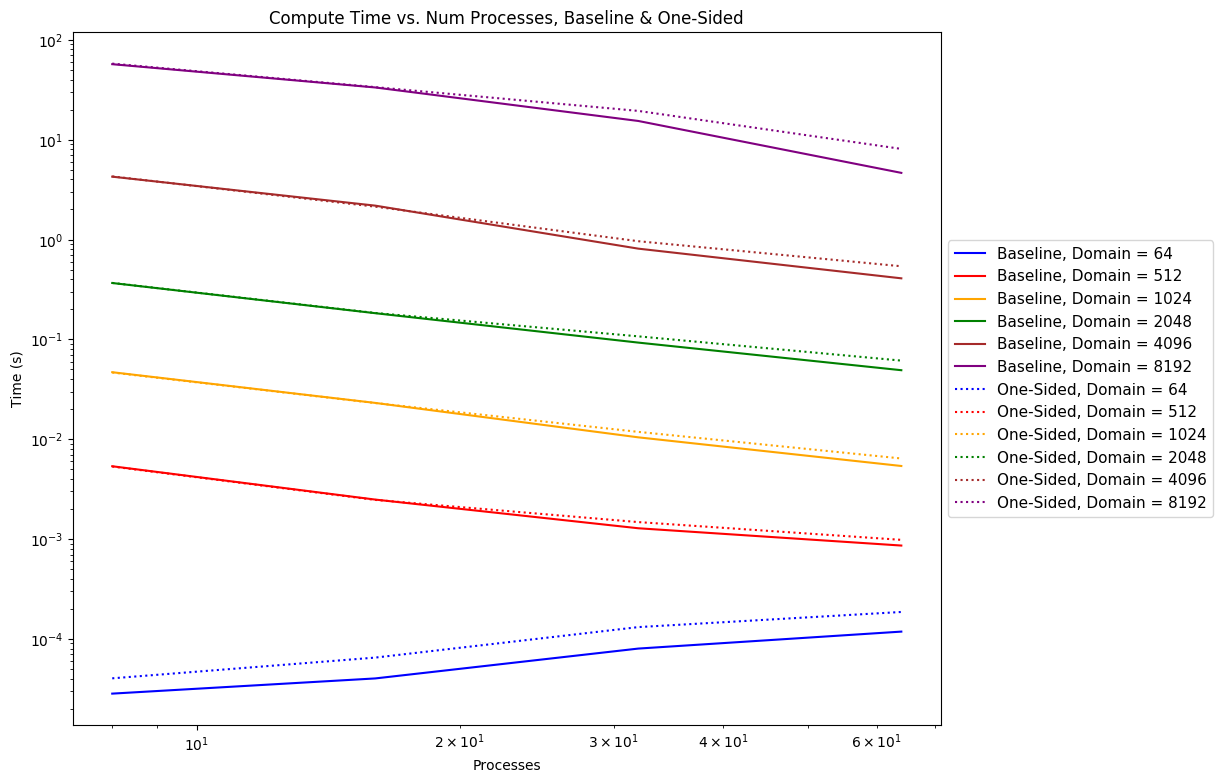
\includegraphics[width=.75\linewidth]{one_sided/compute_multdomain_sandy_os_baseline.png} \\
			(a) Haswell &  (b) Sandy Bridge\\[6pt]
		\end{tabular}
		\caption{Compute Time vs. \#Processes.}
		\label{fig:compute_multdomain_os_baseline}
	\end{figure}
	
	\begin{figure}[h] % h=here, t=top, b=bottom, p=(extra)page, !=force
		\hspace*{-0.25\linewidth}\begin{tabular}{cc}
			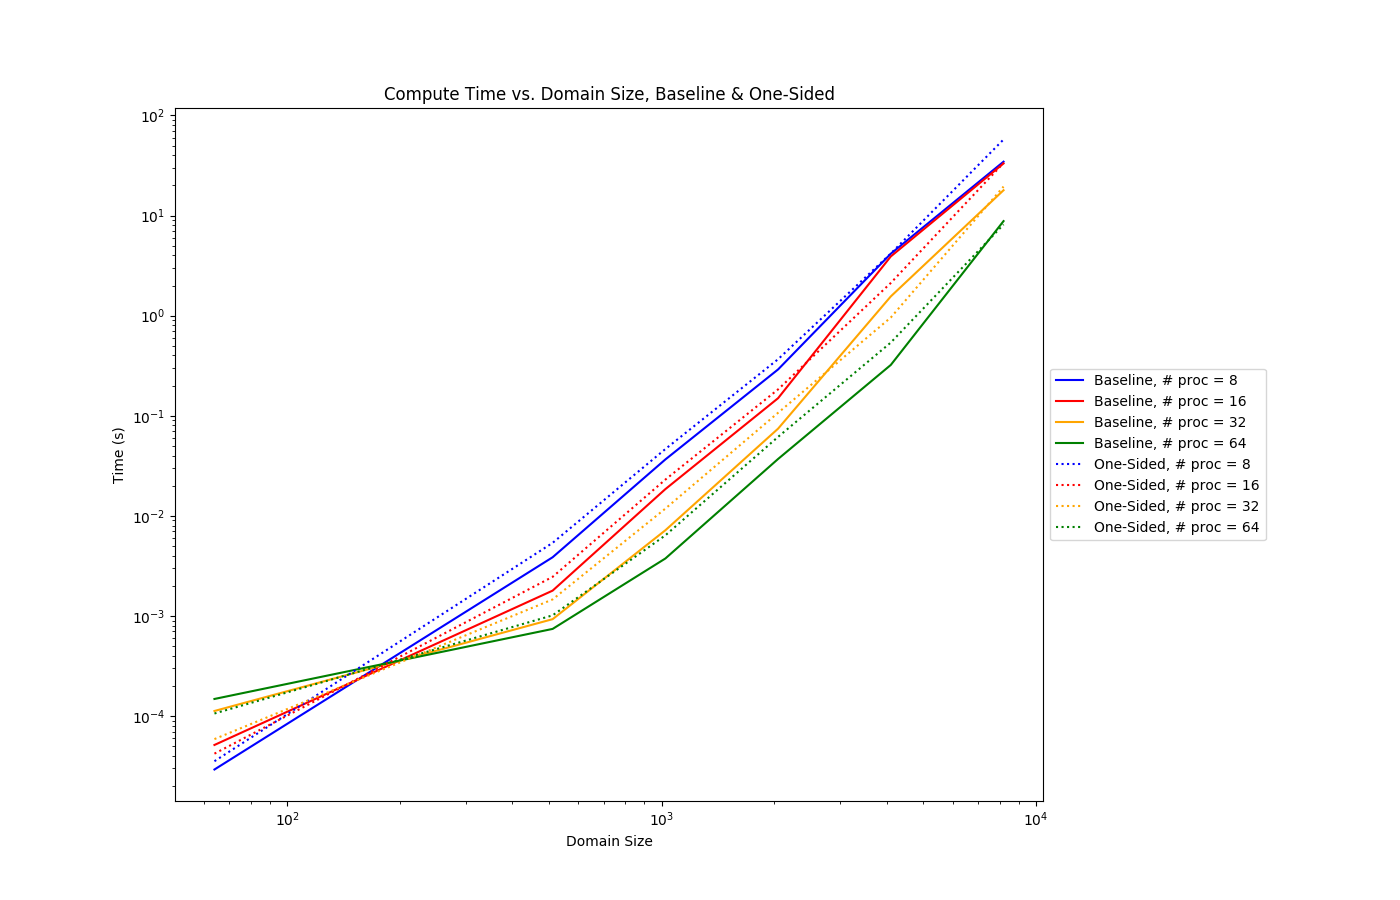
\includegraphics[width=.8\linewidth]{one_sided/compute_multproc_haswell_os_baseline.png} & 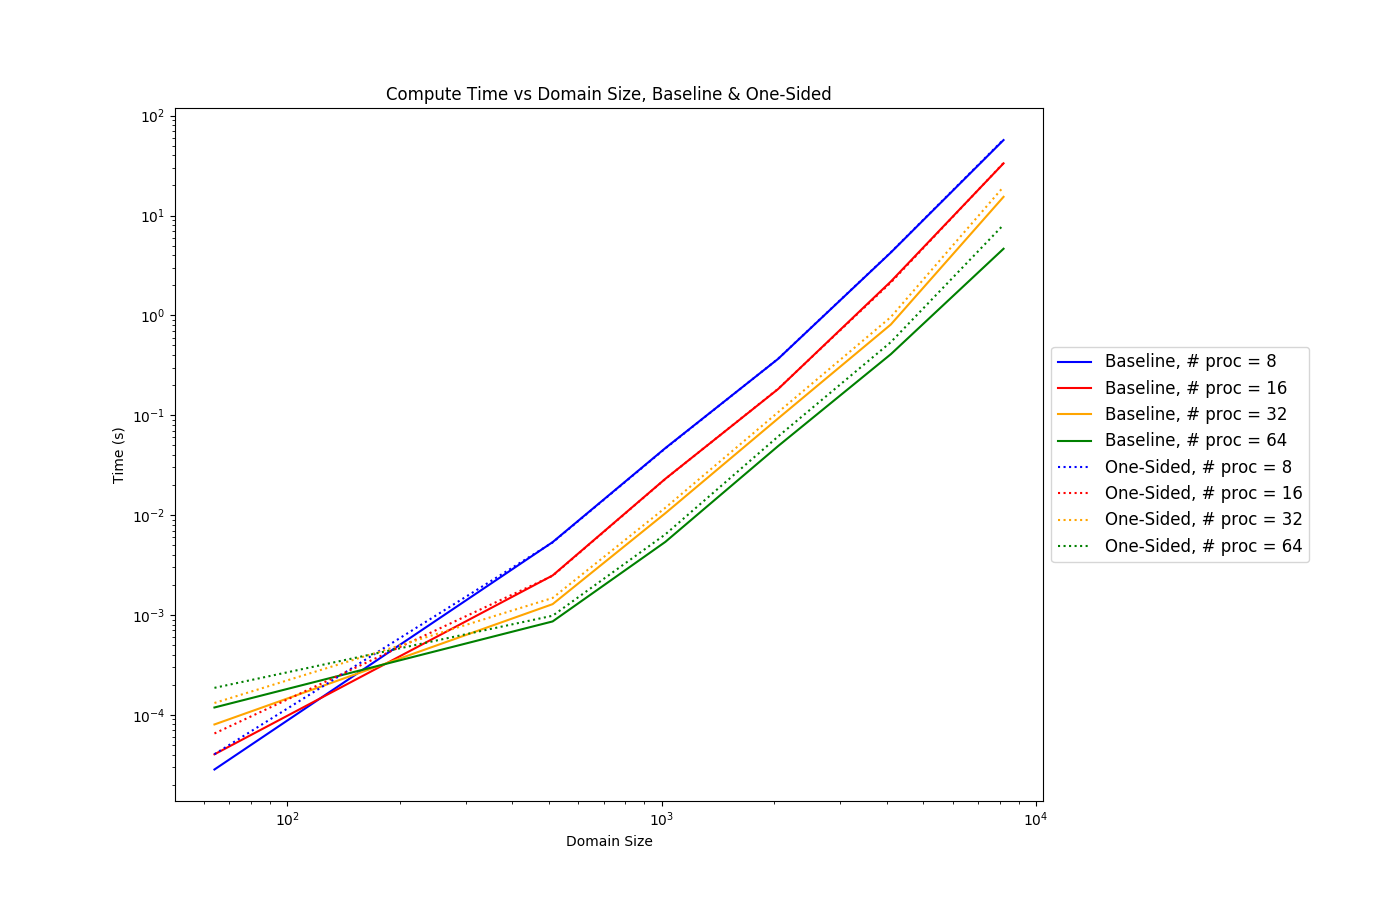
\includegraphics[width=.8\linewidth]{one_sided/compute_multproc_sandy_os_baseline.png} \\
			(a) Haswell &  (b) Sandy Bridge\\[6pt]
		\end{tabular}
		\caption{Compute Time vs. Domain Size.}
		\label{fig:compute_multproc_os_baseline}
	\end{figure}
	
		\begin{figure}[h] % h=here, t=top, b=bottom, p=(extra)page, !=force
		\hspace*{-0.25\linewidth}\begin{tabular}{cc}
			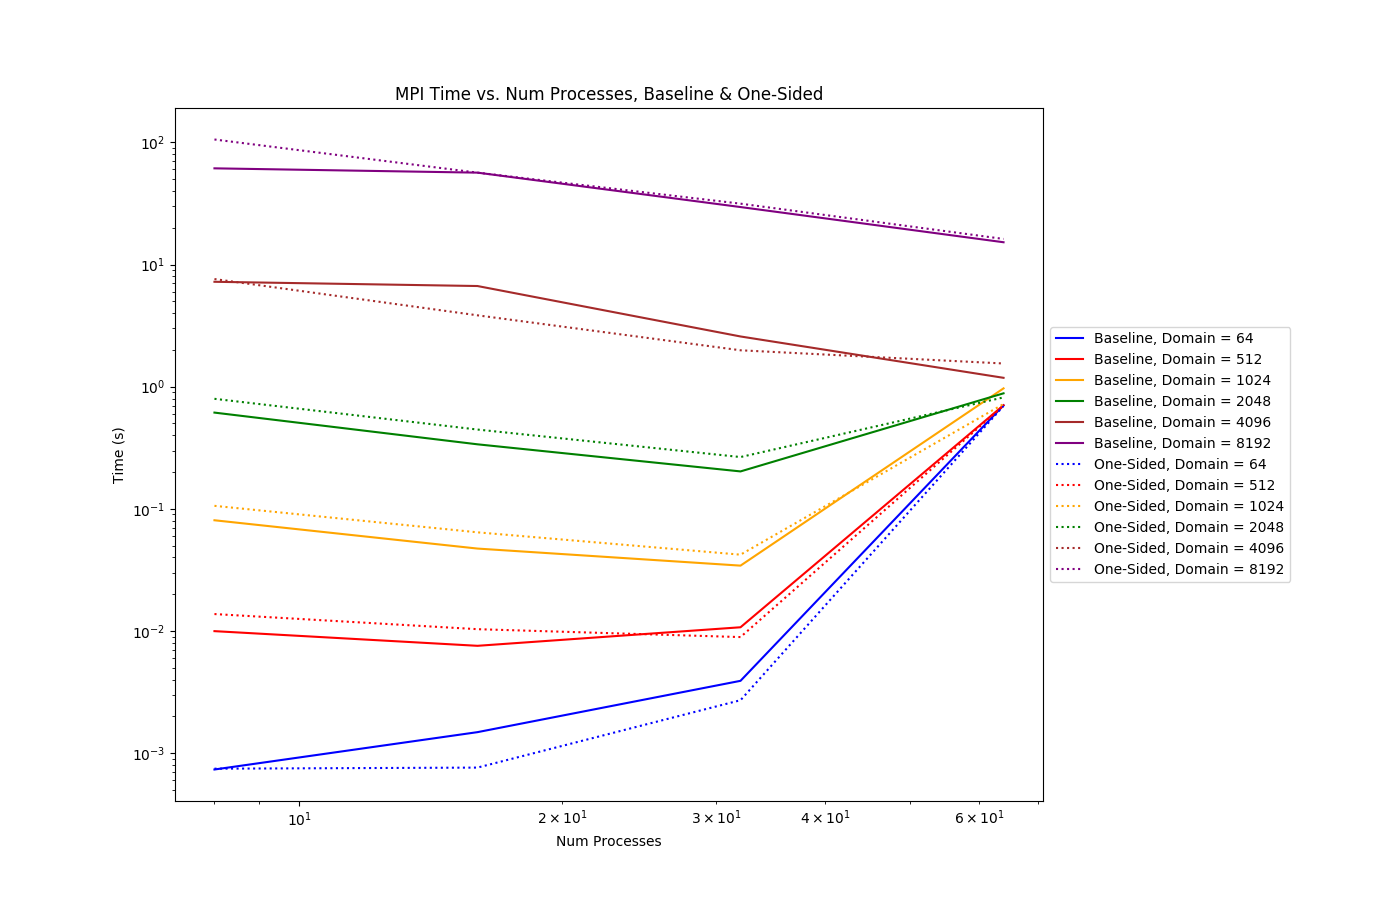
\includegraphics[width=.8\linewidth]{one_sided/mpi_multdomain_haswell_os_baseline.png} & 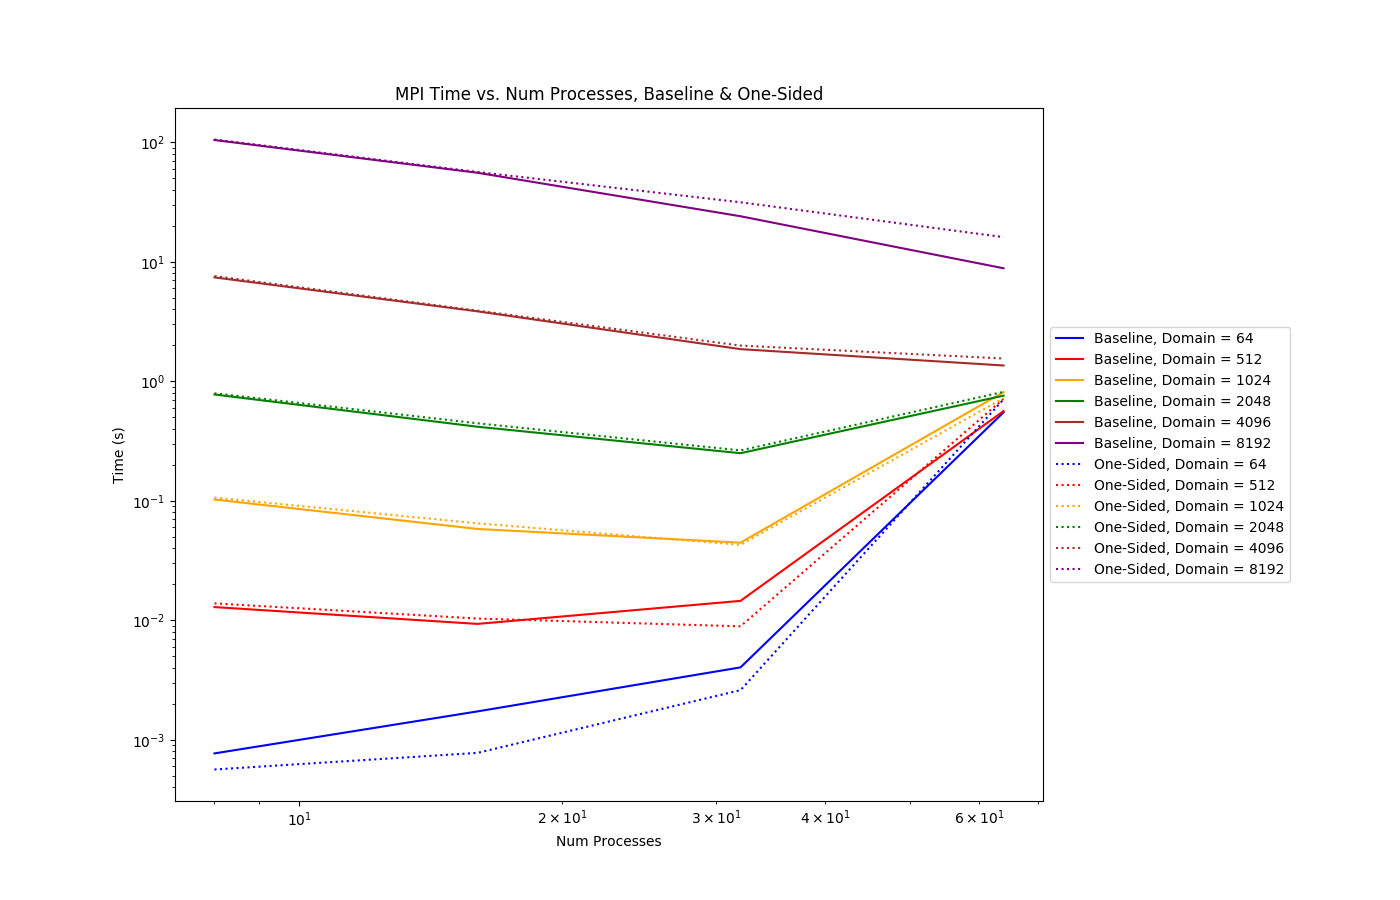
\includegraphics[width=.8\linewidth]{one_sided/mpi_multdomain_sandy_os_baseline.png} \\
			(a) Haswell &  (b) Sandy Bridge\\[6pt]
		\end{tabular}
		\caption{MPI Time vs. \#Processes.}
		\label{fig:mpi_multdomain_os_baseline}
	\end{figure}
	
		\begin{figure}[h] % h=here, t=top, b=bottom, p=(extra)page, !=force
		\hspace*{-0.25\linewidth}\begin{tabular}{cc}
			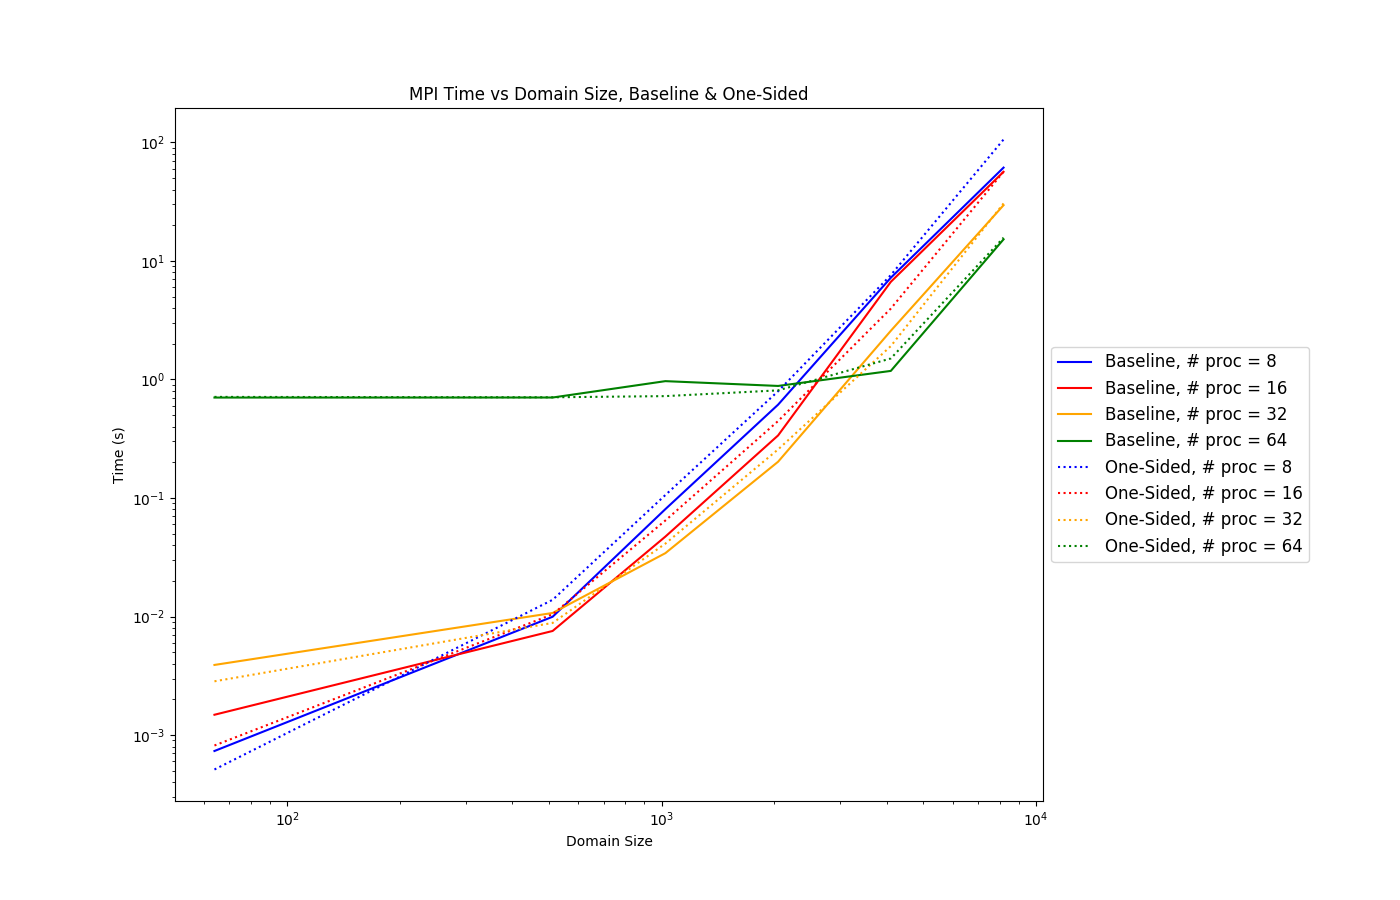
\includegraphics[width=.8\linewidth]{one_sided/mpi_multproc_haswell_os_baseline.png} & 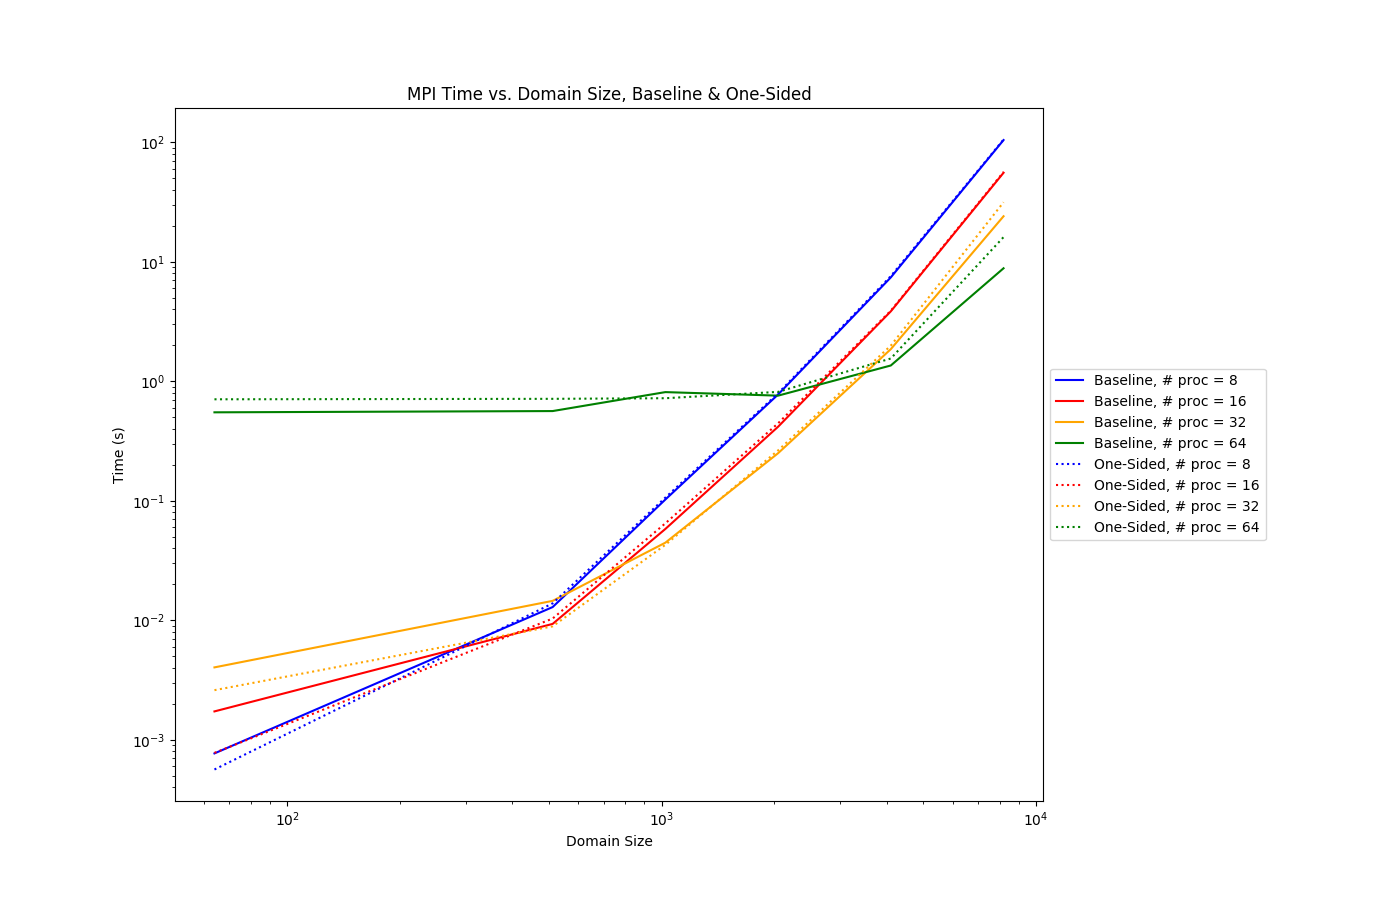
\includegraphics[width=.8\linewidth]{one_sided/mpi_multproc_sandy_os_baseline.png} \\
			(a) Haswell &  (b) Sandy Bridge\\[6pt]
		\end{tabular}
		\caption{MPI Time vs. Domain Size.}
		\label{fig:mpi_multproc_os_baseline}
	\end{figure}
	
			\begin{figure}[h] % h=here, t=top, b=bottom, p=(extra)page, !=force
		\hspace*{-0.25\linewidth}\begin{tabular}{cc}
			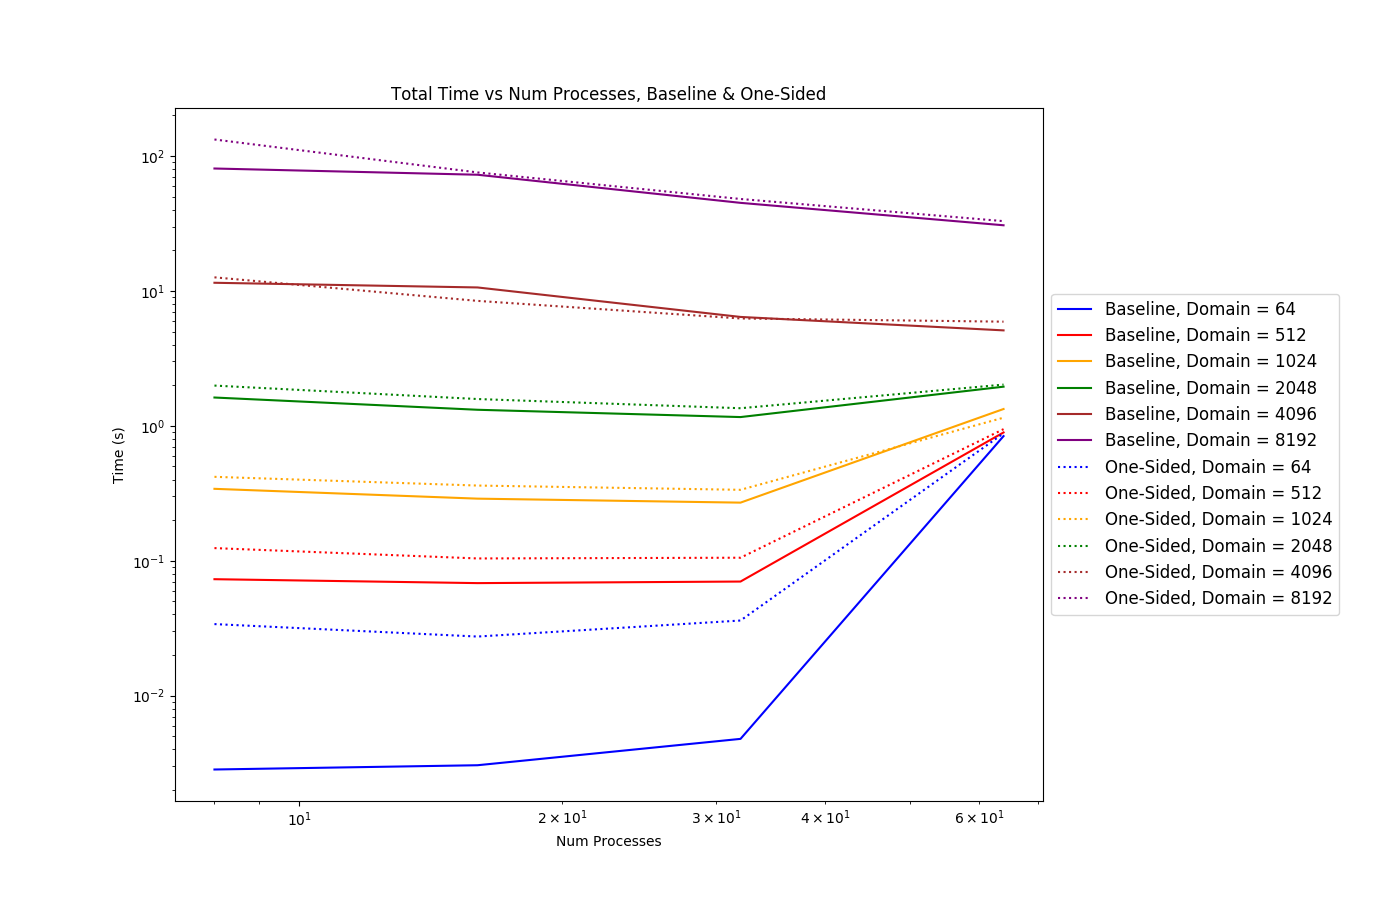
\includegraphics[width=.8\linewidth]{one_sided/total_multdomain_haswell_os_baseline.png} & 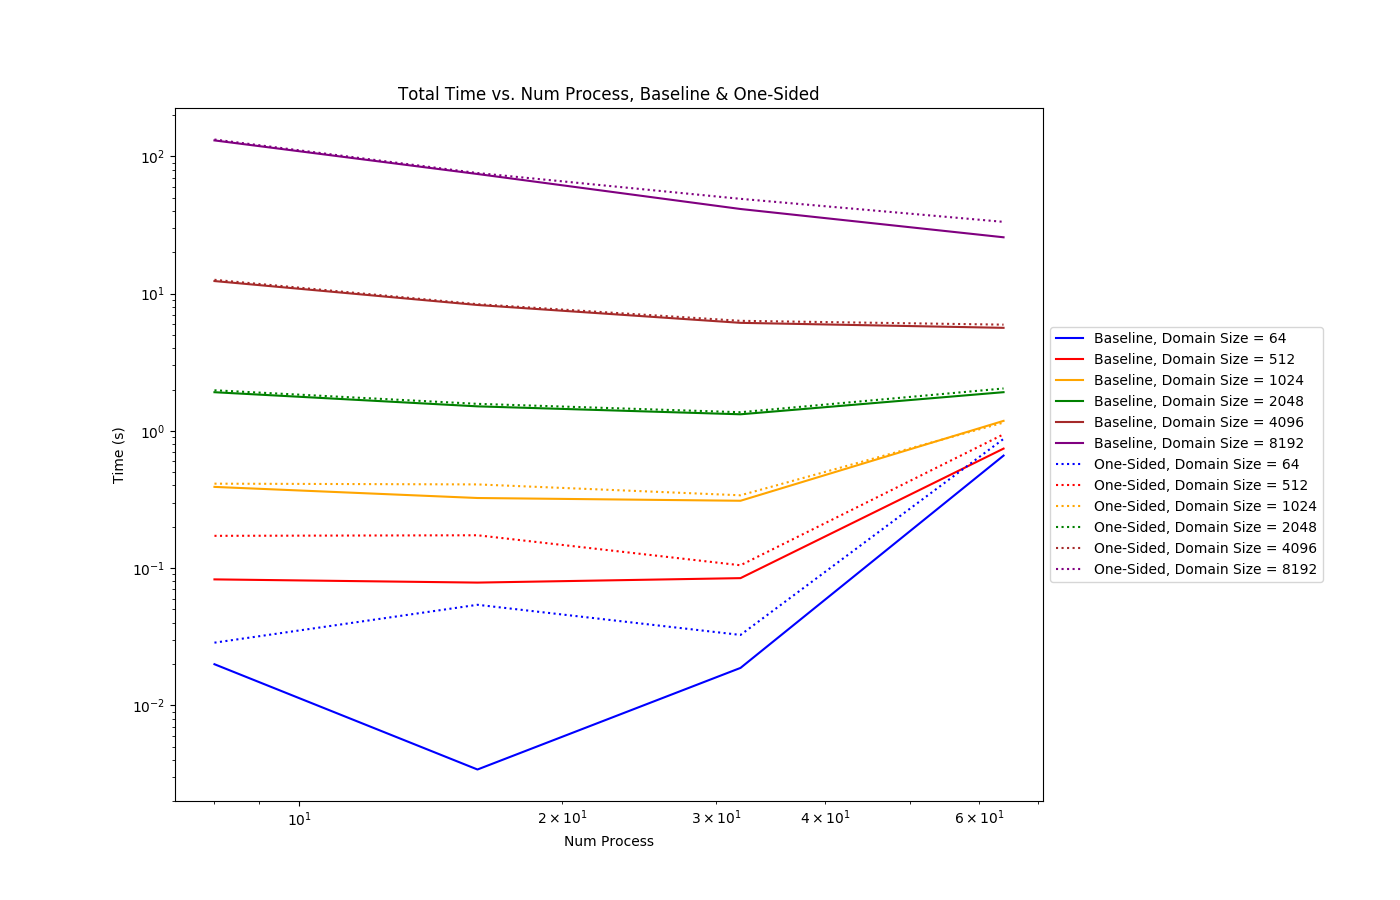
\includegraphics[width=.8\linewidth]{one_sided/total_multdomain_sandy_os_baseline.png} \\
			(a) Haswell &  (b) Sandy Bridge\\[6pt]
		\end{tabular}
		\caption{Total Time vs. \#Processes.}
		\label{fig:total_multdomain_os_baseline}
	\end{figure}
	
		\begin{figure}[h] % h=here, t=top, b=bottom, p=(extra)page, !=force
		\hspace*{-0.25\linewidth}\begin{tabular}{cc}
			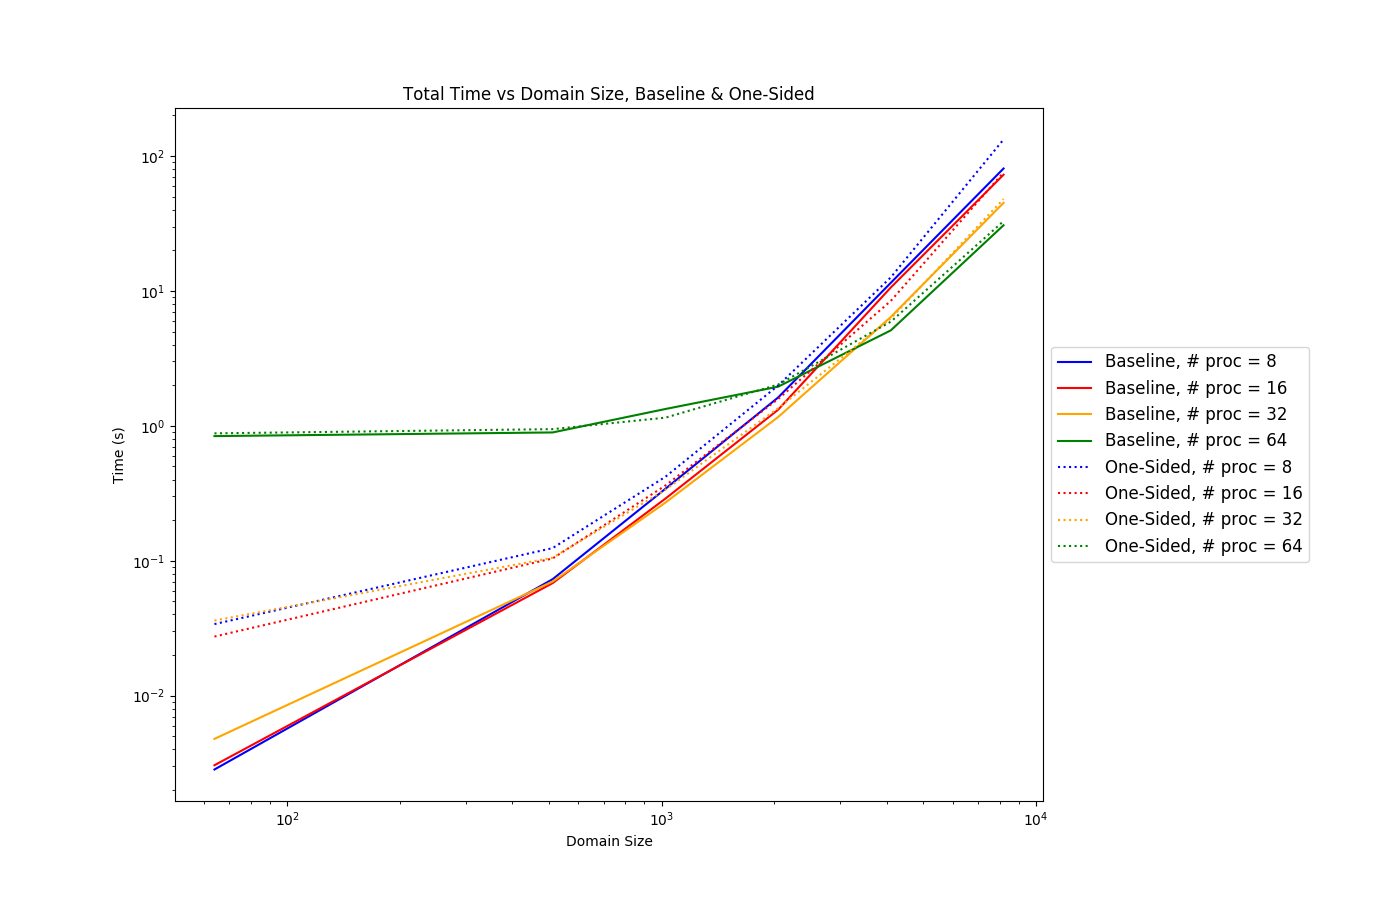
\includegraphics[width=.8\linewidth]{one_sided/total_multproc_haswell_os_baseline.png} & 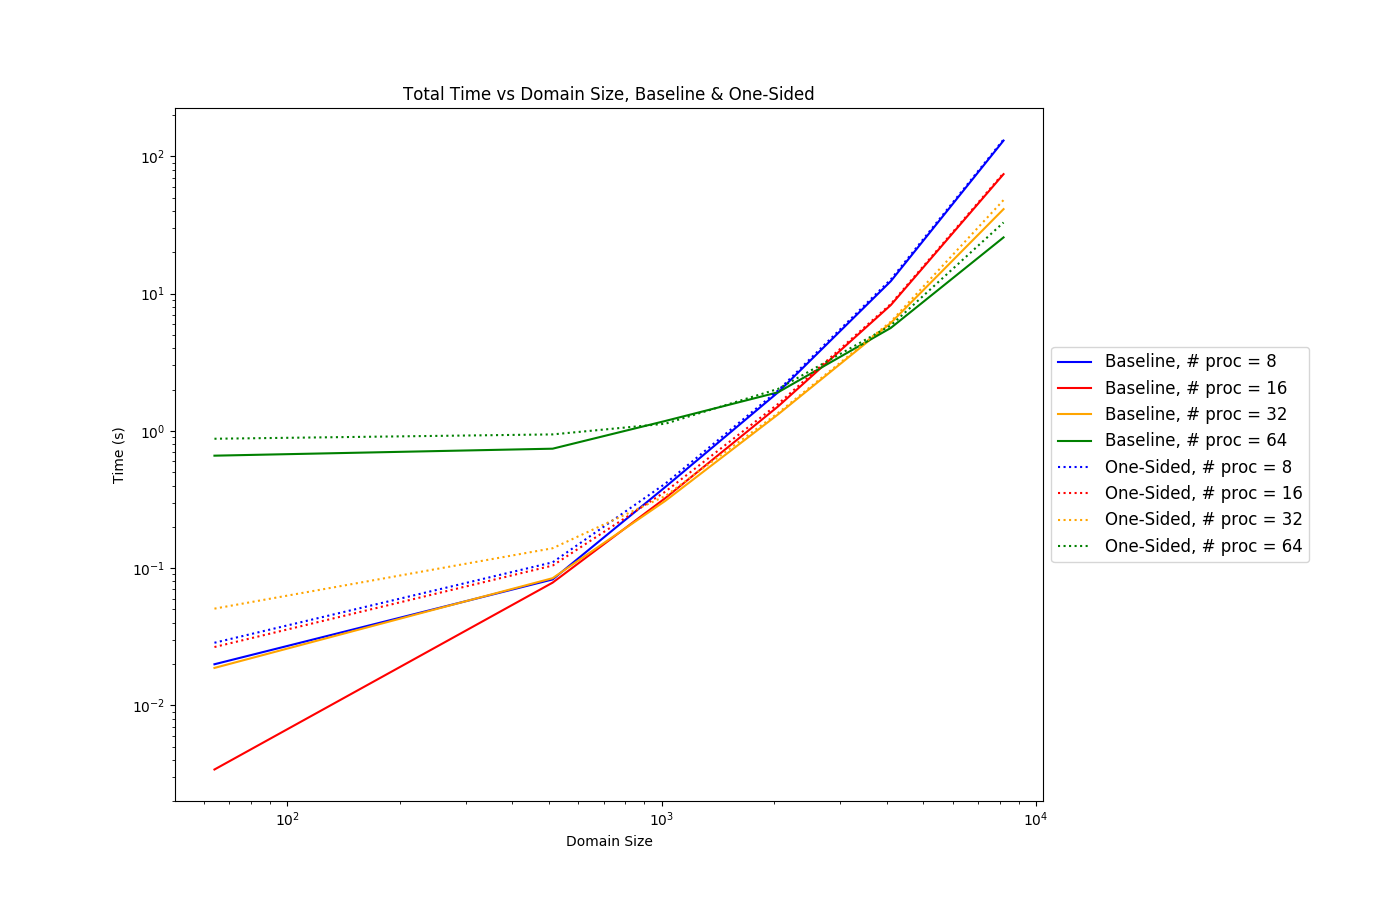
\includegraphics[width=.8\linewidth]{one_sided/total_multproc_sandy_os_baseline.png} \\
			(a) Haswell &  (b) Sandy Bridge\\[6pt]
		\end{tabular}
		\caption{Total Time vs. Domain Size.}
		\label{fig:total_multproc_os_baseline}
	\end{figure}

  \item \hl{Was a speedup observed versus the non-blocking version for the Sandy Bridge and Haswell nodes?}

    \todo{Wait for results of non-blocking}

\end{enumerate}
% % Figure example
% \begin{figure}[p] % h=here, t=top, b=bottom, p=(extra)page, !=force
%    \begin{center}
%      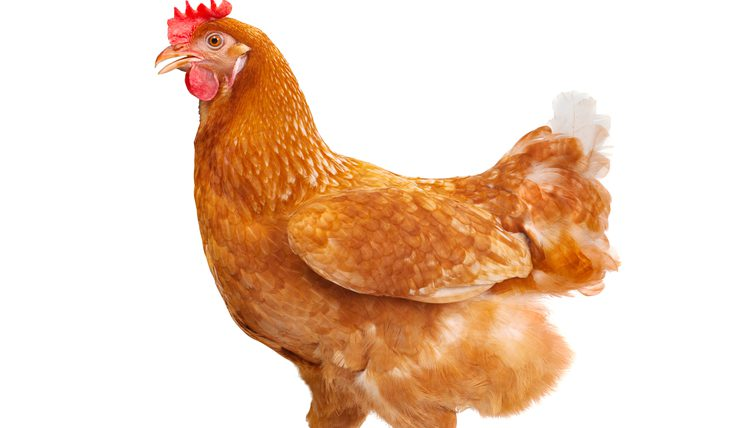
\includegraphics[width=.9\linewidth]{figure.png} % It searches in the Figures/ folder!
%      \caption{Caption text}
%      \label{fig:figureLabelName}
%    \end{center}
% \end{figure}
